\documentclass{article}
\usepackage{graphicx}
\graphicspath{{./figures/}}
\usepackage{mathrsfs}
\usepackage{amsfonts}
\usepackage{amssymb}
\usepackage{amsmath}
\usepackage{subfig}
\title{Using {\it fruitbat} to Investigate Dispersion Measure and Redshift Dependencies for an Intergalactic Medium}
\author{Brad McNiven}
\date{June 2021}

\begin{document}

\maketitle



\section{Introduction}

Fast radio bursts (FRBs) are transient radio pulses which last on the order of a few milliseconds. FRBs are an interesting astronomical phenomenon, as they are of unknown origin and their sources appear to reside outside of the Milky Way galaxy \cite{Petroff}. One of their most interesting features is their abnormally large dispersion measure ($DM$), which is mathematically an integrated density of electrons between the source and the relative observer. Given the exponentially large distances between Earth and interstellar sources of FRBs, $DM$ measurements of a FRB source are extremely difficult given the insufficient resolution of modern telescopes. By instead studying the redshift ($Z$) of a source, which is a doppler relation containing the spectral lines (wavelength) of the source and how it is observed on earth, and $DM$ relations via numeric and analytic means with previously collected astronomical data, one can estimate many other related cosmological effects.

In this project, the third party open source Python package called {\it fruitbat} \cite{fruitbat} is used to calculate this relation between $DM$ and $Z$ via three different methods. Each method uses different sets of cosmological parameters which in turn result in a different numerical result. {\it fruitbat} is used in this project to study the redshift as a function of dispersion measure for a static position in the universe, while also as functions of its latitude and longitude. Since the calculation of both of these quantities allows for one to determine other astronomical properties, we demonstrate this by presenting the comoving and luminosity distance curves as functions of dispersion measure.

\section{Method \& Theory}

The main advantage of {\it fruitbat} is providing a numerical solver for the integral
\begin{equation}
F(Z) = \int_0^Z \frac{dz^{\prime}(1 + z ^\prime )}{\sqrt{\Omega_m(1+z^\prime)^3 + \Omega_{\Lambda} (1+z^\prime)^{3(1-w)}}},
\label{eq:integral}
\end{equation}
where $Z$ is the redshift, $\Omega_m$ is the cosmic matter density, $\Omega_\Lambda$ is the cosmic dark energy density, and $w$ is the dark energy equation of state parameter. The utility of this is that if one can numerically determine $F(Z)$, one can also calculate a variety of interesting and fundamental cosmological quantities given its direct relation to $DM$. This in turn means one now has the ability to study FRBs by inputting an estimated redshift and additional set of input cosmological parameters. 

For this project, we use {\it fruitbat} to determine Eqn \ref{eq:integral} and use three separate methods to study the impact of different cosmological parameters on the dispersion measure, redshift, and associated properties.

In the first method, referred to here as Zhang2018 \cite{Zhang2018}, all existing baryons present in the universe are fully ionized, while 85\% of them exist in the intergalactic medium. Moreover, there is a 0.875-to-1 ratio of electrons and baryons in the universe. This results in a dispersion measure equal to 
\begin{equation}
    DM=\frac{3cH_0\Omega_b\chi f_{igm} }{8\pi G m_p}F(Z),
\end{equation}
where $c$ is the speed of light, $H_0$ is the Hubble constant, $\Omega_b$ is the cosmic baryon density,  $\chi$ is the free electron per baryon, $f_{igm}$ is the fraction of baryons in the intergalactic medium, $G$ is the gravitational constant, and $m_p$ is the proton mass.

The second method, referred to as Ioka2003 \cite{Ioka2003}, assumes that all baryons in the universe are ionized, and there is a 1-to-1 ratio of electrons to baryons throughout. Thus, its dispersion measure is 
\begin{equation}
    DM=\frac{3cH_0 \Omega_b}{8\pi G m_p} F(Z).
\end{equation}

The third method investigated, referred to as Inoue2004 \cite{Inoue2004}, assumes that helium is singly ionized while hydrogen is fully ionized, resulting in the dispersion measure
\begin{equation}
    DM=9.2\times10^{-10}c H_0 \Omega_b F(Z).
\end{equation}
It is noted that all calculations performed were done so using the Planck18 comological parameter set \cite{Planck2018}, where $H_0=67.66$, $\Omega_b=0.04897$, $\Omega_m=0.3111$, $\Omega_\Lambda=0.6874$, and $w=-1$.

{\it fruitbat} was used by first intializing the \emph{fruitbat.Frb()} function where a dispersion measure range was used (0-5000) was fed into the function along with the specific method used for each calculation via \emph{method="methodX"}. Additional parameters were called into the function when specifying specific latitude and longitude coordinates via \emph{gl=X} and \emph{gb=Y}, respectively. Once a numerical result is obtained, the redshift was then obtained using the \emph{calc\_redshift()} function, followed by any other properties dependent on $Z$. In particular, the redshift dependent comoving and luminosity functions can be called in once the redshift is calculated by using the functions \emph{calc\_comoving\_distance()} and \emph{calc\_luminosity\_distance()} respectively. Note these two functions return {$\langle$\emph{astropy.units.quantity.Quantity}$\rangle$} datatypes, meaning one must provide \emph{.value} at the end of the function call to store the numerical result.

\section{Results and Discussion}

\subsection{Redshift Dispersion Measure Relation}

We first present the redshift as a function of dispersion measure for a given FRB for each of the three methods, with no specification on spatial positioning, shown in Fig \ref{fig:ZvDM}. From the figure, it is apparent that each method deviates from one another with increasing $DM$, however Zhang2018 and Inoue2004 are much closer in agreement. For a $DM$ of $\sim5000$ pc cm$^{-3}$, $Z$ obtained via Ioka2003 is only $\sim65\%$ of that obtained by Zhang2018.  

\begin{figure}[!htb]
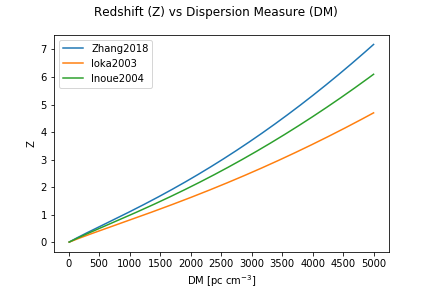
\includegraphics[width=\linewidth]{Z_vs_DM.png}
\caption{Redshift as a function of dispersion measure for the Zhang2018, Ioka2003 and Inoue2004 methods.}
\label{fig:ZvDM}
\end{figure}

With knowledge of $Z$, many other properties can now be investigated. We demonstrate this by calculating the comoving distance, which is the distance between the FRB source and earth without factoring in the expansion of the universe. This is mathematically defined as
\begin{equation}
d_C(Z)=\frac{c}{H_0} \int_0^Z \frac{dz^\prime}{ \sqrt{\Omega_r (1+z^\prime)^4 +\Omega_m (1+z^\prime)^3 + \Omega_\Lambda}  },
\end{equation} 
where $\Omega_r$ is the radiation density. We can also look at the luminosity distance, a quantity relating the apparent and absolute magnitude of the FRB source, defined as
\begin{equation}
d_L(Z)=(1+Z)d_C(Z).
\end{equation}


\begin{figure}[!htb]
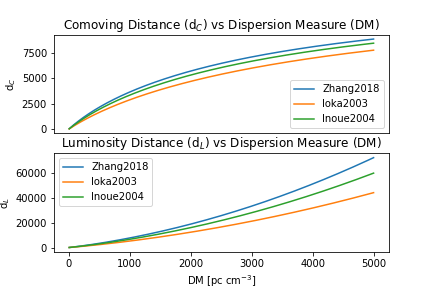
\includegraphics[width=\linewidth]{distance_vs_DM.png}
\caption{comoving and luminosity distances as functions of dispersion measure for the Zhang2018, Ioka2003, and Inoue2004 methods. }
\label{fig:distance_v_DM}
\end{figure}

Fig \ref{fig:distance_v_DM} presents these distance curves as functions of dispersion measure. From the figure, it is clear there is deviation as $DM$ increases, however the curves associated with the Zhang2018 and Inoue2004 methods are again very close even for $DM\sim5000$ pc cm$^{-3}$. An interesting trend is that as $DM\rightarrow0$,  these two methods produce the same $d_C$ for $DM \leqslant 600$ pc cm$^{-3}$ and $d_L$ for $\leqslant 1200$ pc cm$^{-3}$.

\subsection{Specified Coordinate Results}

Fig \ref{fig:heatmapDM} presents the dispersion measure for a given set of latitude and longitude coordinates ranging from -$90^\circ-90^\circ$. Results shown in the figure were obtained by specifying the \emph{dm} parameter in the \emph{fruitbat.Frb()} function to be 600. This means the observed dispersion measure does not have Milky Way or host galaxy contributions subtracted from it. This was then passed to \emph{calc\_dm\_galaxy()} to calculate the dispersion measure contribution of only the Milky Way for each of the three methods.

\begin{figure}[!htb]
\centering
\subfloat[]{\label{a}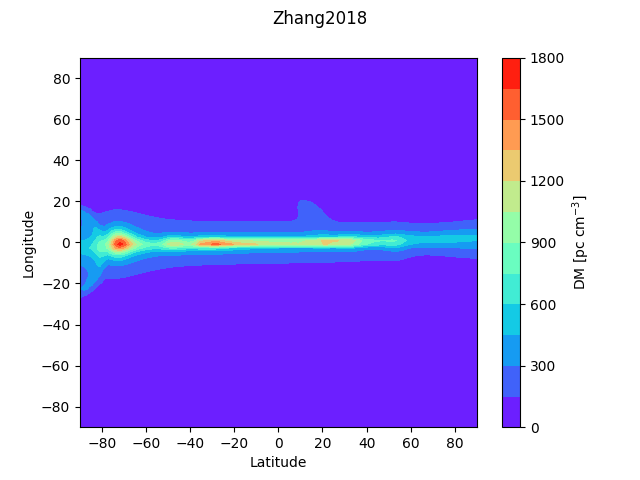
\includegraphics[width=.5\linewidth]{DM_heatplot_Zhang2018.png}}\hfill
\subfloat[]{\label{b}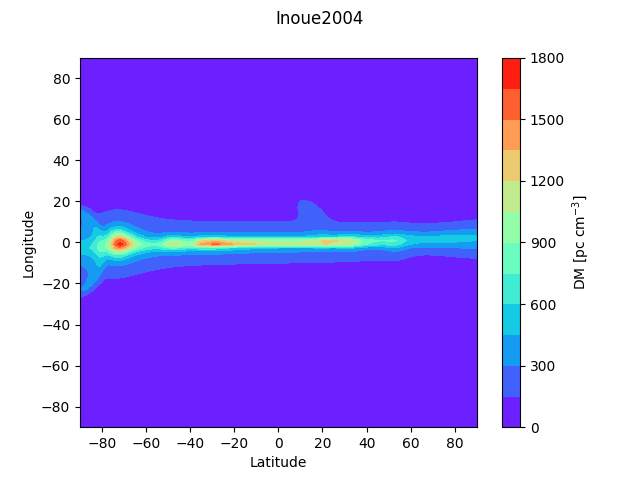
\includegraphics[width=.5\linewidth]{DM_heatplot_Inoue2004.png}}\par 
\subfloat[]{\label{c}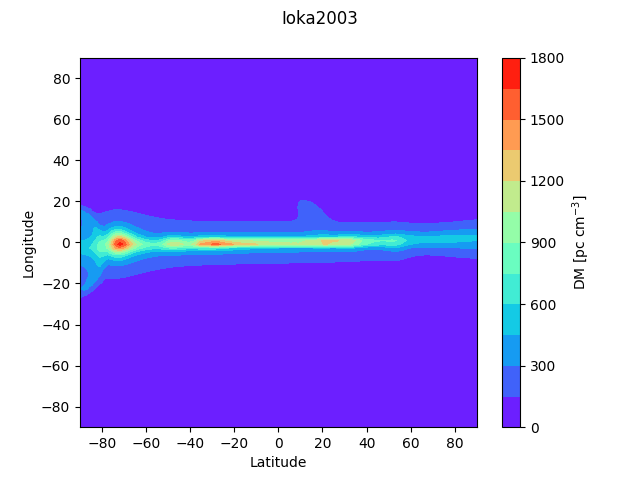
\includegraphics[width=.5\linewidth]{DM_heatplot_Ioka2003.png}}
\caption{Heatmap depicting the dispersion measure for latitude and longitude coordinates for the Zhang2018, Ioka2003 and Inoue2004 methods.}
\label{fig:heatmapDM}
\end{figure}

From the figure, we see that each of the three methods appears to result in the same dispersion measure over the range of probed latitude and longitude coordinates. This could be due to the fundamental handling of dispersion measure Milky Way contributions in each method, or that the defined grid space was high enough resolution. Given the data is probed on a 100$\times$100 grid, the resolution could be further increased by a factor of 10 to determine whether any structure change occurs between either of the three methods.

\begin{figure}[!htb]
\centering
\subfloat[]{\label{a}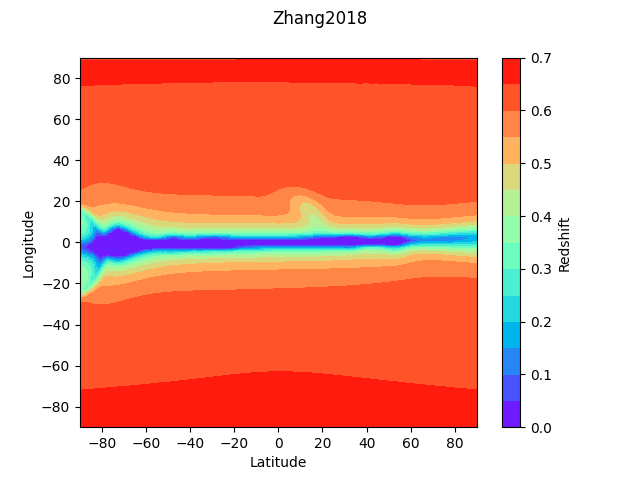
\includegraphics[width=.5\linewidth]{redshift_heatplot_Zhang2018.png}}\hfill
\subfloat[]{\label{b}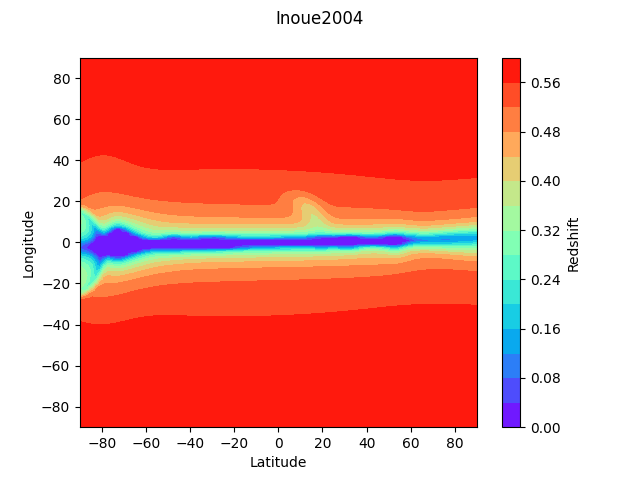
\includegraphics[width=.5\linewidth]{redshift_heatplot_Inoue2004.png}}\par 
\subfloat[]{\label{c}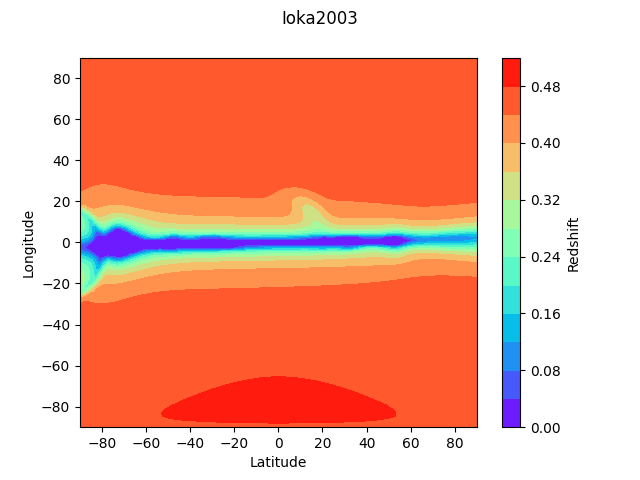
\includegraphics[width=.5\linewidth]{redshift_heatplot_Ioka2003.png}}
\caption{Heatmap depicting the redshift for latitude and longitude coordinates for the Zhang2018, Ioka2003 and Inoue2004 methods.}
\label{fig:heatplotZ}
\end{figure}

We also look at the redshift for a given set of latitude and longitude coordinates, shown in the heatmap presented in Fig \ref{fig:heatplotZ}. Here we see that all probed latitude coordinates confined within a longitude range of -$20^\circ-20^\circ$ results in the same structure, however different structure appears outside of these bounds for each method. 

We look to study these structural differences further by performing a ``cut'' in the heatplot, with the latitude fixed at -$0.909^\circ$. This result is shown in Fig \ref{fig:heatplotcut}, along with a cut from Fig \ref{fig:heatmapDM} at the same fixed latitude for completeness.

\begin{figure}[!htb]
\centering
\subfloat[]{\label{a}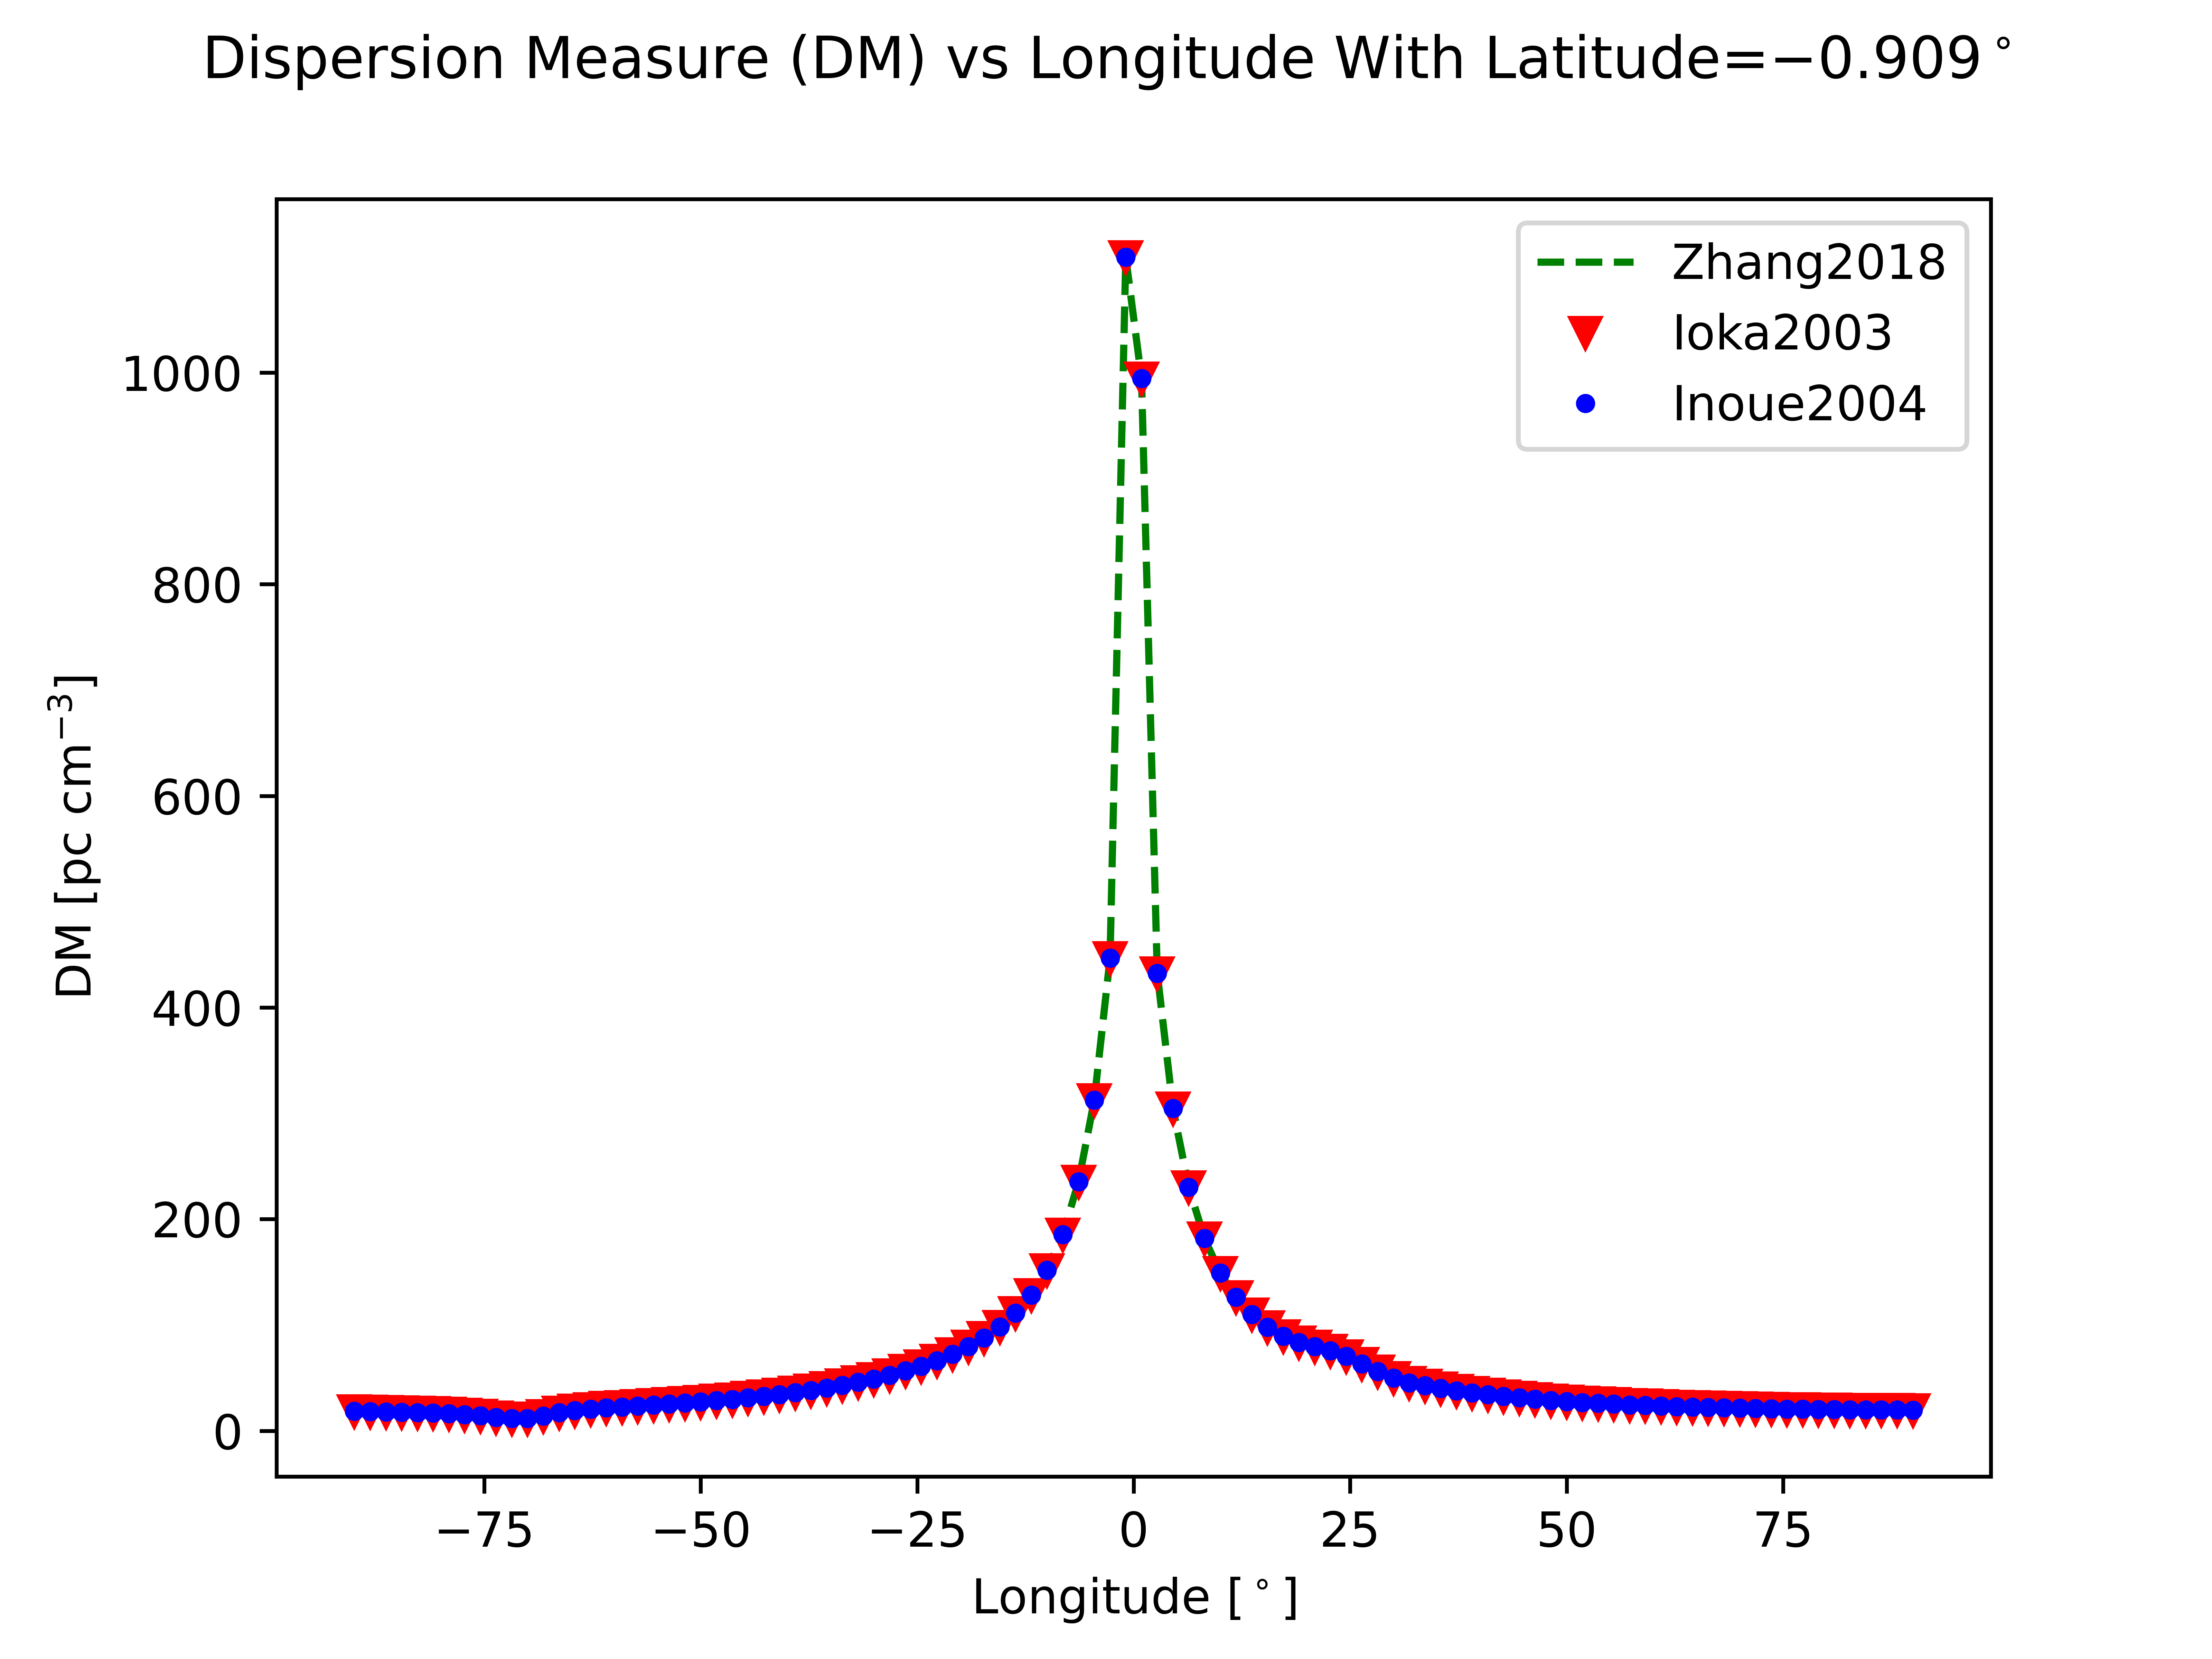
\includegraphics[width=.5\linewidth]{DM_vs_longitude.png}}\hfill
\subfloat[]{\label{b}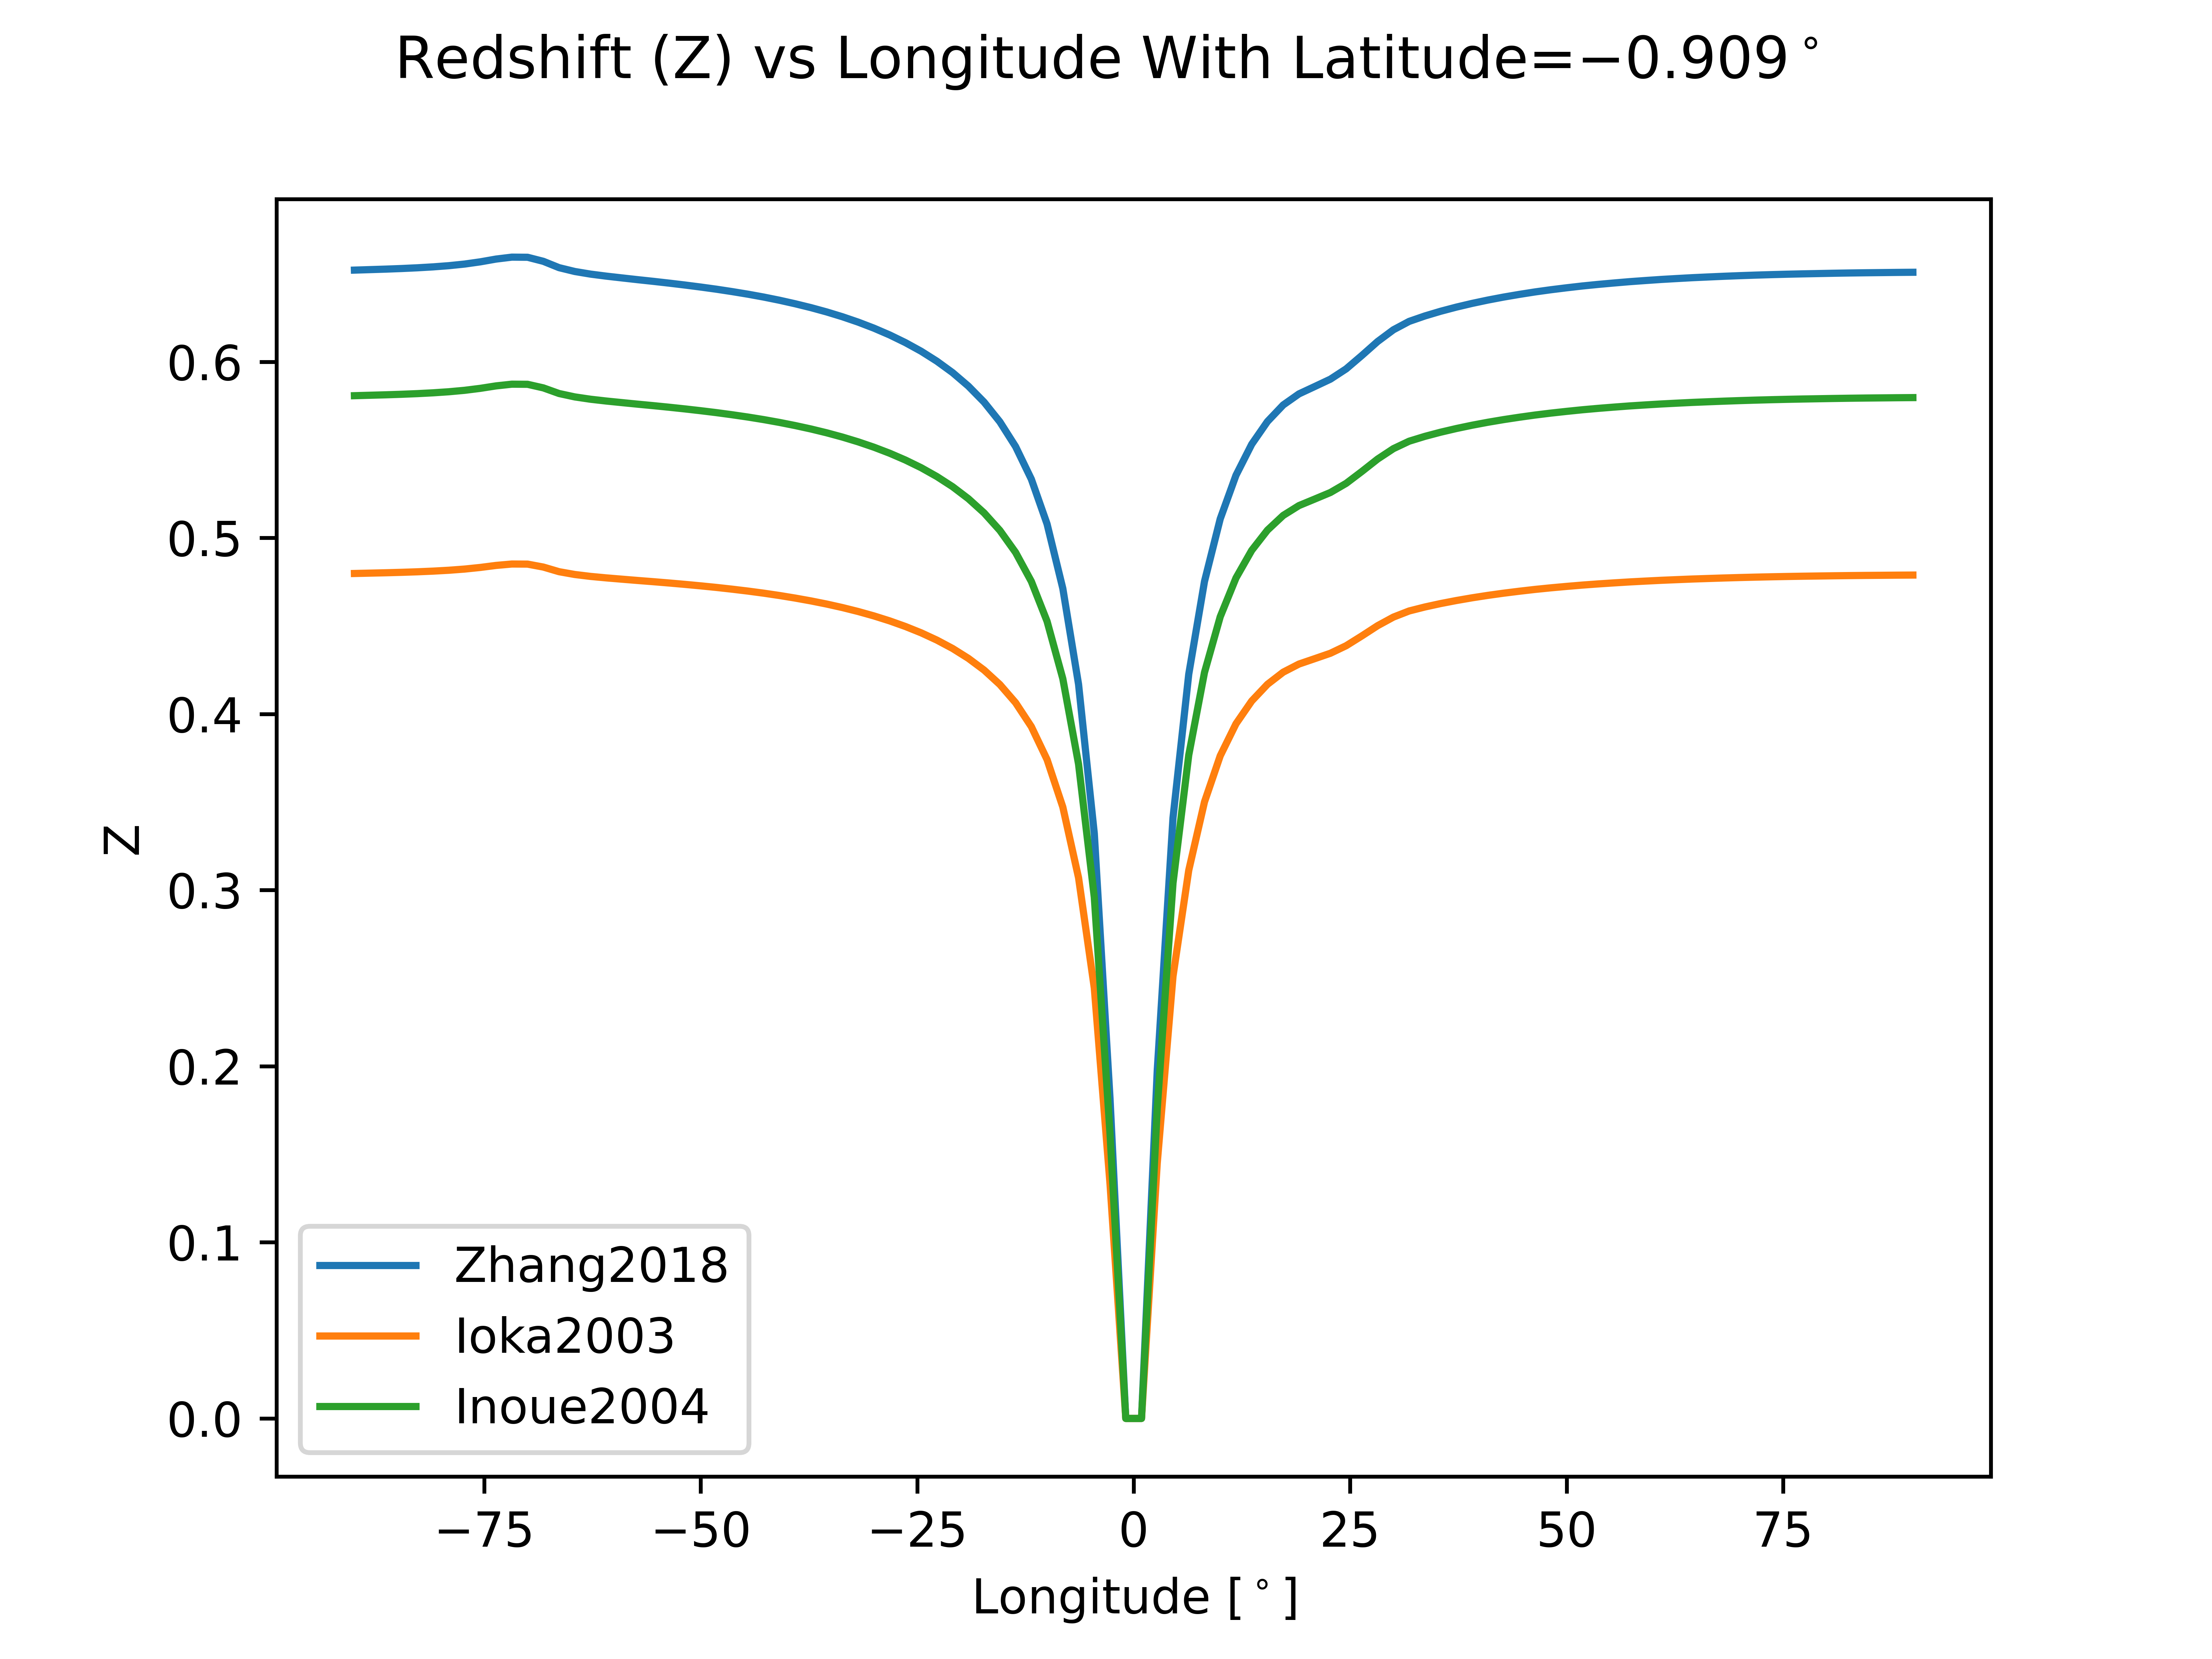
\includegraphics[width=.5\linewidth]{Z_vs_longitude.png}}
\caption{ (a) dispersion measure and (b) redshift as functions of longitude for the Zhang2018, Ioka2003 and Inoue2004 methods.}
\label{fig:heatplotcut}
\end{figure}

From Fig \ref{fig:heatplotcut}(a), we find that the three methods do in fact to produce the same exact results when calculating dispersion measures contributions from only the Milky Way. Conversely, Fig \ref{fig:heatplotcut}(b) produces different structure between the three methods for longitudes outside of -$20^\circ-20^\circ$. Similar discontinuous bumps appear on each of the curves but appear at different longitudes, indicating each of the three methods produce different redshifts for specific coordinates even with the same dispersion measure contributions.

\section{Conclusion}

In this project, the third party open source package \emph{fruitbat} was used to determine the relation between dispersion measure and redshift for the the methods Zhang2018, Ioka2003, and Inoue2004, which differ based on the universal assumptions made. Redshift as a function of dispersion measure curves were produced for each method where differences in each of the three curves was observed. These redshift values were used to then calculate the differences in their comoving and luminosity distances. The coordinate specification power of the \emph{fruitbat} package was also exploited, such that the dispersion measure and associated redshift from the Milky Way were investigated over a range of latitude and longitude coordinates. These results were shown as heatplots, where the dispersion measure was found to be the same for each method while the redshift was found to differ for longitudinal coordinates outside of the range -$20^\circ-20^\circ$. These differences were further investigated by cuts taken of each heatmap, near a latitude of $0^\circ$.

\bibliographystyle{ieeetr}
\bibliography{refs}
\end{document}
